\documentclass[11pt]{standalone}

\usepackage{helvet}

\usepackage{ifthen}
\usepackage{tikz} 
\usetikzlibrary{shapes.misc}
\usetikzlibrary{arrows,arrows.meta}
\usetikzlibrary{calc,intersections, patterns, math}

\definecolor{pfeil}{RGB}{168,167,167}
\definecolor{petrol}{RGB}{0, 118, 136}
\definecolor{darkgoldenrod}{RGB}{184, 134, 11}
\colorlet{petrol-lighter}{petrol!40}
\colorlet{darkgoldenrod-lighter}{darkgoldenrod!40}

\begin{document}

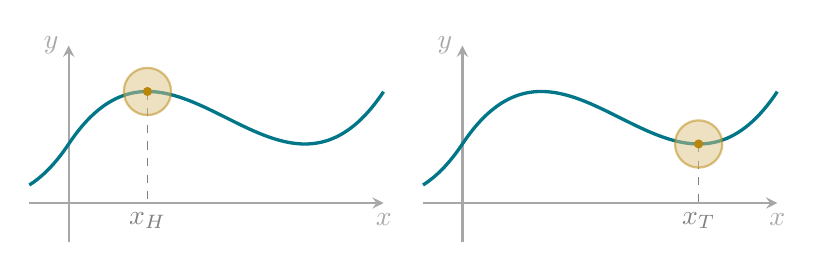
\begin{tikzpicture}[pfeil]

    % \draw[thick, fill=petrol!20, draw=petrol-lighter, rounded corners=2ex, opacity=0.5] (0,0) rectangle ++ (1.5,3.5);
    % \draw[thick, fill=darkgoldenrod!20, draw=darkgoldenrod-lighter, rounded corners=2ex, opacity=0.5] (5,0) rectangle ++ (1.5,3.5);

        \draw[thick, -stealth] (-0.5,0) -- (4,0) node[below] {$x$};
        \draw[thick, -stealth] (0,-0.5) -- (0,2) node[left] {$y$};
        \draw[very thick, petrol, domain=-0.5:4, samples = 100] plot(\x,{1/6*\x^3-1*\x^2+1.5*\x+0.75}) ;
        \draw[dashed, gray] (1,2.83333*0.5) -- (1,0) node[below] {$x_H$};
        \draw[darkgoldenrod,fill=darkgoldenrod!50, opacity=0.5,thick] (1,2.83333*0.5) circle (0.3);
        \draw[darkgoldenrod,fill] (1,2.833333*0.5) circle (0.05);

        \begin{scope}[xshift=5cm]
            \draw[thick, -stealth] (-0.5,0) -- (4,0) node[below] {$x$};
				\draw[thick, -stealth] (0,-0.5) -- (0,2) node[left] {$y$};
				\draw[very thick, petrol, domain=-0.5:4, samples = 100] plot(\x,{1/6*\x^3-1*\x^2+1.5*\x+0.75}) ;
				\draw[dashed, gray] (3,1.5*0.5) -- (3,0) node[below] {$x_T$};
				\draw[darkgoldenrod,fill=darkgoldenrod!50, opacity=0.5,thick] (3,1.5*0.5) circle (0.3);
				\draw[darkgoldenrod,fill] (3,1.5*0.5) circle (0.05);
        \end{scope}

\end{tikzpicture}

\end{document}
